
\documentclass[12pt]{article}
\usepackage{amsmath}
\DeclareMathOperator*{\argmin}{arg\,min} % thin space, limits underneath in displays
\DeclareMathOperator*{\argmax}{arg\,max} % thin space, limits underneath in displays
\newtheorem{thm}{Theorem}
\usepackage{amssymb}
\usepackage{amsfonts}
\usepackage{mathrsfs}
\usepackage{bm}
\usepackage{indentfirst}
\setlength{\parindent}{0em}
\usepackage[margin=1in]{geometry}
\usepackage{graphicx}
\usepackage{setspace}
\doublespacing
\usepackage[flushleft]{threeparttable}
\usepackage{booktabs,caption}
\usepackage{float}
\usepackage{graphicx}

\usepackage{import}
\usepackage{xifthen}
\usepackage{pdfpages}
\usepackage{transparent}

\newcommand{\incfig}[1]{%
\def\svgwidth{\columnwidth}
\import{./figures/}{#1.pdf_tex}
}




\usepackage{graphicx}
\usepackage{xspace,color}
\usepackage{url}
\usepackage{listings}


\lstset{commentstyle=\color{gray},keywordstyle=\color{black},
showstringspaces=false, basicstyle = \small
} %% basicstyle set fontsize
\lstnewenvironment{rc}[1][]{\lstset{language=R}}{}
\newcommand{\ri}[1]{\lstinline{#1}}  %% Short for 'R inline'



\lstdefinelanguage{language=R}{
numbers=left,
numberstyle=\footnotesize,
numbersep=1em,
xleftmargin=1em,
framextopmargin=2em,
framexbottommargin=2em,
showspaces=false,
showtabs=false,
showstringspaces=false,
frame=l,
tabsize=4,
}











\title{Something you need to know}
\author{Synferlo}
\date{May. 4, 2021}


\begin{document}
\maketitle
\newpage





\section{Sampling Distribution}

\subsection{Std. deviation vs. Std. error}
Two important parameters in each distribution: mean, standard deviation.

Given the sample data, we want to estimate the distribution of the 
population, i.e., want to know which distribution generate the data.

By estimating the distribution, we estimate the mean and the std 
deviation. The estimated std deviation of a sampling distribution is
referred to as a {\underline {std error.}}

\begin{equation*}
\text{ Std. deviation } = \sqrt {\text{ variance }}
\end{equation*}


\subsection{Estimate sampling distribution}
Mean of the sampling distribution should be the same as the true mean,
$ \mathbb{E}(\mu_{X}) = \mu $. And the std. error, $ s_{X} $:
\begin{equation*}
s_{X} = \sqrt { \frac{\text{ variance }}{n}} = 
\sqrt { \frac{\sigma^{2}}{n}} = \frac{\sigma}{\sqrt {n}}
\end{equation*}



Suppose we generate a sample, with size 5, 
from $ Normal(\mu = 22, \sigma^{2} = 1.5^{2}) $,
the standard error for the sampling distribution would be
\begin{equation*}
s_{X} = \frac{\sigma}{\sqrt {n}} = \frac{1.5}{\sqrt {5}} \approx 0.671
\end{equation*}

Then we can use R to plot the sampling and true distribution.

\begin{figure}[H]
\caption{Sampling vs. True distribution}
\center{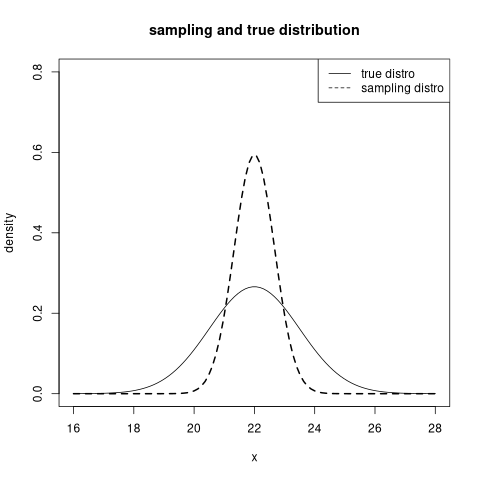
\includegraphics[scale =.5 ]  {figures/sampling_vs_true_distribution.png}}
\end{figure}


Clearly, the sampling distribution is taller and skinner, while the
true distribution is flatter.





\subsubsection{Confident Interval for the mean}

By doing this, must assume the data is normally distributed.

Then,

Step 1: Compute sample mean, $ \mu_{X} $ and std deviation, $ s_{X}$. 
(page 394 in Tilman's R code book)

Step 2: Compute sample std. error. 
\begin{equation*}
		se = \frac{s_{X}}{\sqrt {n}}
\end{equation*}


Step 3: Since we assume obs are normally distributed and we are using
$ s_{X} $ rather $ \sigma_{X} $, t-distribution with $ n - 1 $ degree
of freedom is the appropriate method, where $ n $ is the sample size.


Step 4: Choose the confident interval, e.g., 95\% . It says 
$ \alpha = 0.05 $. Hence the {\underline {critical value}} is 
\begin{equation*}
\text{ cumulative probability } = 1 - \frac{\alpha}{2} = 0.975
\end{equation*}
Now we have the cumulative probability, p, for the qt() function in R.
We can use the following code to compute the critical value (or called
the quantile value in R).

\noindent\fbox{%
\parbox{\textwidth}{%

$ \alpha $ = 0.975\\
\#You need to substitute n by the actual sample size.\\
critical\_value  = qt(p = $ \alpha $, df = n - 1) \\
print(critical\_value)\\
\#it is the value on the horizontal axis, if you plot the density
of t-distribution.

}%
}\\

So the area within the confidence interval(CI) is $ prob. = .95 $

\begin{figure}[H]
		\center{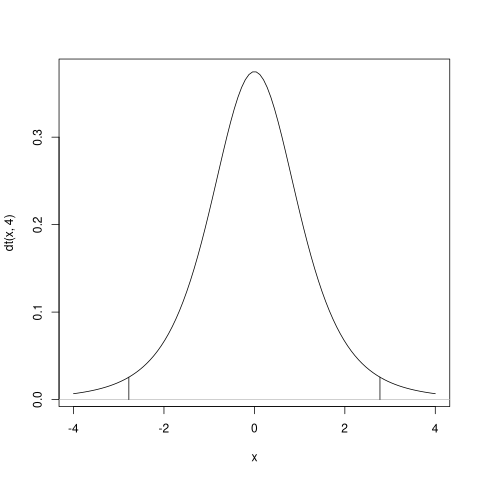
\includegraphics[scale = 0.5 ]  {figures/confidence_interval.png}}
\end{figure}


Step 5: Now you have sample mean ($ \mu_{X} $), std error ($ se $), 
and the critical value for .95 confidence interval. Then you can 
make the following inference:

\noindent\fbox{%
\parbox{\textwidth}{%

I am in 95\% confidence saying that the true mean of the population
lies somewhere between
\begin{equation*}
\mu_{X} - se  \times \text{ critical\_value } <
\quad \mu \quad < \mu_{X}  + se  \times \text{ critical\_value }
\end{equation*}
}%
}\\






\section{Hypothesis Test}
\subsection{null and alternative hypothesis}
\subsubsection{Null Hypo.}
Null Hypothesis: $ H_0 $. The claim that is assumed to be true.

\subsubsection{Alt. Hypo.}
All. hypo.: $ H_1 $. The conjecture that you are testing for, against
the null.

Three types of tests based on different $ H_1 $:

1. lower-tailed test: When $ H_1 $ is defined in terms of a less-than
statement, with $ < $. It is {\underline {one-sided}}.

2. upper-tailed test: When $ H_1 $ is defined in terms of a greater-than
statement, with $ > $. It is {\underline {one-sided}}.

3. two-tailed test: When $ H_1 $ is defined in terms of a different-to
statement, with $ \ne $. It is {\underline {two-sided}}.










\subsection{Test statistics}

The statistic that is compared to the appropriate standardized
sampling distribution to yield the $ p $-value.


\subsection{$ p $-value}

The meaning for $ p $-value in different types of test:

1. In a lower-tailed test: $ p $-value is a left-hand tail probability
from the sampling distribution of interest.

2. In an upper-tailed test: a right-hand tail prob. 

3. In two-sided test, the sum of left and right tail probability.
This is equivalent to two times the area in one tail when the
sampling distribution is {\underline {symmetric}}.\\




Consider and example:


\begin{figure}[H]
		\center{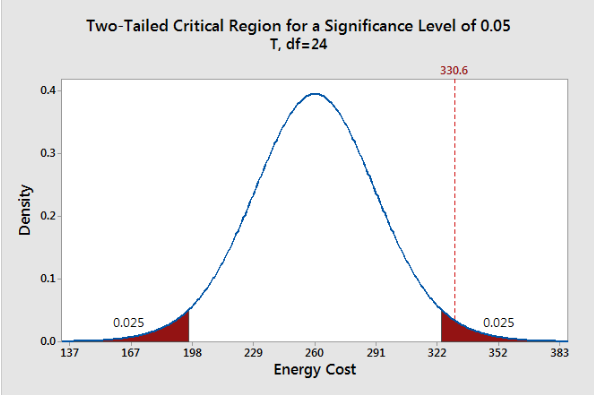
\includegraphics[scale =.5 ]  {figures/CI_95.png}}
		{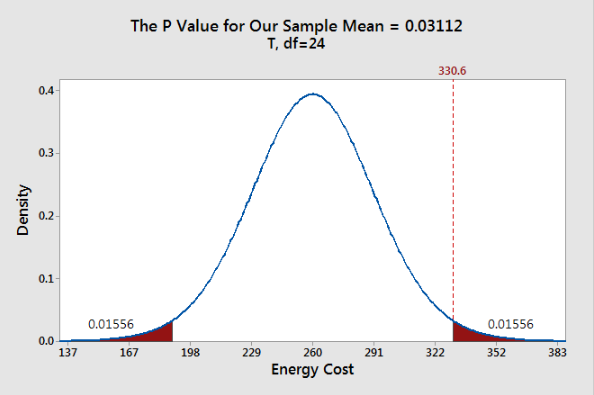
\includegraphics[scale =.5 ]  {figures/pvalue_against_CI.png}}
\end{figure}

$ H_0 $: the population mean is 260\\
$ H_1 $: the population mean differs from 260

After calculation, we get the sample mean is $ 330.6 $

Red area in the left figure stands for the area of our 95\% CI.
Clearly, our sample mean is outside the CI.

Red area in the right figure stands for the $ p $-value for this sample
mean. Note, we can compute this by using pnorm() in R.
The $ p $-value says the prob. of obtaining a {\underline {sample mean}}
that is as extreme (or even far away from the true mean, 260) as what
we got (330.6) is $ 0.01556  \times 2 = 0.03112 $.


Clearly, when the sample mean appears outside the 95\% CI, the
$ p $-value is also less than the significance level, 
$ 0.03112 < 0.05 $. Or we say 
{\underline {$ p $-value is less than the significance level}}.


Since our sample mean is outside the 95 CI, we CANNOT say that
the population mean is 260 with 95\% confidence. That's why we 
{\underline {reject the null when $ p $-value $ < $ the 
significance level.}}


Remember, $ p $-value is calculated based on the position of your
sample mean. If the $ p $-value is less than the significance level, 
{\underline {your sample mean is outside the CI}}. Hence, we 
reject the null.


\subsection{Comments on Hypothesis Test}

1. $ p $-value never provides ``proof" of either $ H_0 $ or $ H_1 $ being
{\underline {truly}} correct.

Rejecting $ H_0 $ merely implies that {\underline {the sample data
suggest $ H_1 $ ought to be preferred.}}\\










\subsection{Testing Means}

How to test the mean with t-test? Let's do this.


Suppose you have a sample from the population with mean = 80. You
want to test if the true mean, i.e., population mean, is 80 with 95
confidence.

\begin{align*}
H_0: \mu &= 80\\
H_1: \mu &\le 80
\end{align*}



By doing this, we need to:

step 1: compute sample mean($  \overline{X} $) and the sample std 
deviation, or SD in short ($ s $).\\
mean = $ 80.10174 $, SD = $ s $ = $ 1.651756 $.
\\

step 2: compute test statistic T:
\begin{equation*}
T = \frac{ \overline{X} - \mu}{s/\sqrt {n}} \approx 0.3895706
\end{equation*}	
The dashed line stands for t = 0.3895706.
Note, the sample SD, $ s/\sqrt {n} $, is the estimated standard 
error of the mean.

T follows a t-distribution with $ n - 1 $ degree of freedom.\\

step 3: Note, $ H_1 $ suggests that this is a left-tailed test. So,
the $ p $-value is provided as the area under the sampling distribution
(a t-distribution with DOF = 39) to the left of a vertical line at T.

Now, compute the $ p $-value = $ 0.6505133 $. It says the area at the
left side of the dashed line is about 0.65 (The cumulative prob.).


step 4: Compare the $ p $-value with significance level, $ \alpha $.
Clearly, $ p $-value is much greater than 0.05. 
{\underline {We fail to reject the null}}. It pretty much makes sense
because the sample we use is generated from a normal distribution with
mean = 80. It is very unlikely we can reject the null. The code is 
below.

\begin{figure}[H]
		\center{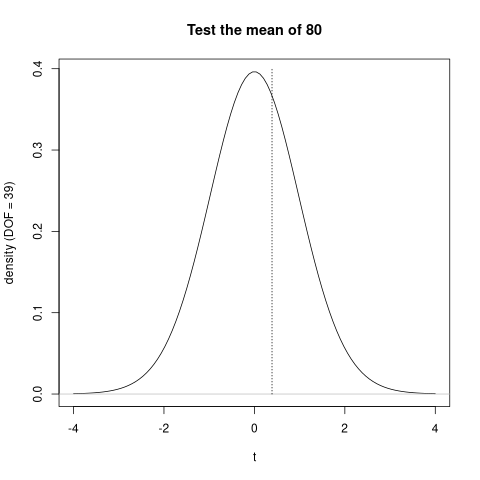
\includegraphics[scale =.5 ]  {figures/t-test.png}}
\end{figure}









\begin{rc}
 
# generate a sample
n = 40
# make sure we have the same generated numbers, set the seed
set.seed(5)
sample = rnorm(n, 80, 1.5)
# compute the sample mean and SD
sample_mean = mean(sample)			# X = [1] 80.10174
# sample SD: s
sample_sd = sd(sample)				# s = [1] 1.651756
sample_se = sample_sd/sqrt(n)	# [1] 0.2611655

# T statistics:
sample_T = (sample_mean - 80)/sample_se		# [1] 0.3895706

# compute the p-value, i.e., the cumulative prob. using pt()
# remember, sample_T is t value on the horizontal axis of the density.
sample_p_value = pt(sample_T, n-1)		# [1] 0.6505133

# Clearly, p-value is much greater than 0.05. We fail to reject 
# the null.

\end{rc}
























\end{document}

